\documentclass[11pt,oneside]{article}
\usepackage[T1]{fontenc}
\usepackage[utf8]{inputenc}
% \usepackage{lmodern}
%\usepackage[adobe-utopia,uppercase=upright,greeklowercase=upright]{mathdesign}
\usepackage[adobe-utopia]{mathdesign}
%\usepackage{minionpro}
% \usepackage{pifont}
% \usepackage{amssymb}
\usepackage{amsmath}
\usepackage[francais]{babel}
% \usepackage[francais]{varioref}
\usepackage[dvips]{graphicx}

\usepackage{framed}
\usepackage[normalem]{ulem}
\usepackage{fancyhdr}
\usepackage{titlesec}
\usepackage{vmargin}
\usepackage{longtable}

\usepackage{ifthen}


%\usepackage{epsfig}
\usepackage{subfig}

\usepackage{multirow}
\usepackage{multicol} % Portions de texte en colonnes
\usepackage{flafter}%floatants après la référence



\usepackage{color}
\usepackage{colortbl}


\definecolor{gris25}{gray}{0.75}
\definecolor{bleu}{RGB}{18,33,98}
\definecolor{bleuf}{RGB}{42,94,171}
\definecolor{bleuc}{RGB}{231,239,247}
\definecolor{rougef}{RGB}{185,18,27}
\definecolor{rougec}{RGB}{255,230,231}
\definecolor{vertf}{RGB}{103,126,82}
\definecolor{vertc}{RGB}{220,255,191}

\newenvironment{rem}[1][\hsize]%
{%
    \def\FrameCommand
    {%
\rotatebox{90}{\textit{\textsf{Remarque}}} 
        {\color{bleuf}\vrule width 3pt}%
        \hspace{0pt}%must no space.
        \fboxsep=\FrameSep\colorbox{bleuc}%
    }%
    \MakeFramed{\hsize#1\advance\hsize-\width\FrameRestore}%
}%
{\endMakeFramed}%


\newenvironment{savoir}[1][\hsize]%
{%
    \def\FrameCommand
    {%
\rotatebox{90}{\textit{\textsf{Savoir}}} 
        {\color{bleuf}\vrule width 3pt}%
        \hspace{0pt}%must no space.
        \fboxsep=\FrameSep\colorbox{bleuc}%
    }%
    \MakeFramed{\hsize#1\advance\hsize-\width\FrameRestore}%
}%
{\endMakeFramed}%

\newenvironment{prob}[1][\hsize]%
{%
    \def\FrameCommand%
    {%
\rotatebox{90}{\textit{\textsf{ Problématique}}} 
        {\color{rougef}\vrule width 3pt}%
        \hspace{0pt}%must no space.
        \fboxsep=\FrameSep\colorbox{rougec}%
    }%
    \MakeFramed{\hsize#1\advance\hsize-\width\FrameRestore}%
}%
{\endMakeFramed}%

\newenvironment{obj}[1][\hsize]%
{%
    \def\FrameCommand%
    {%
\rotatebox{90}{\textit{\textsf{ $\;$}}} 
        {\color{rougef}\vrule width 3pt}%
        \hspace{0pt}%must no space.
        \fboxsep=\FrameSep\colorbox{rougec}%
    }%
    \MakeFramed{\hsize#1\advance\hsize-\width\FrameRestore}%
}%
{\endMakeFramed}%

\newenvironment{defi}[1][\hsize]%
{%
    \def\FrameCommand%
    {%
\rotatebox{90}{\textit{\textsf{Définition\\}}} 
        {\color{bleuf}\vrule width 3pt}%
        \hspace{0pt}%must no space.
        \fboxsep=\FrameSep\colorbox{bleuc}%
    }%
    \MakeFramed{\hsize#1\advance\hsize-\width\FrameRestore}%
}%
{\endMakeFramed}%


\newenvironment{hypo}[1][\hsize]%
{%
    \def\FrameCommand%
    {%
\rotatebox{90}{\textit{\textsf{Hypothèse\\}}} 
        {\color{bleuf}\vrule width 3pt}%
        \hspace{0pt}%must no space.
        \fboxsep=\FrameSep\colorbox{bleuc}%
    }%
    \MakeFramed{\hsize#1\advance\hsize-\width\FrameRestore}%
}%
{\endMakeFramed}%


\newenvironment{prop}[1][\hsize]%
{%
    \def\FrameCommand%
    {%
\rotatebox{90}{\textit{\textsf{Propriété\\}}} 
        {\color{bleuf}\vrule width 3pt}%
        \hspace{0pt}%must no space.
        \fboxsep=\FrameSep\colorbox{bleuc}%
    }%
    \MakeFramed{\hsize#1\advance\hsize-\width\FrameRestore}%
}%
{\endMakeFramed}%

\newenvironment{props}[1][\hsize]%
{%
    \def\FrameCommand%
    {%
\rotatebox{90}{\textit{\textsf{Propriétés\\}}} 
        {\color{bleuf}\vrule width 3pt}%
        \hspace{0pt}%must no space.
        \fboxsep=\FrameSep\colorbox{bleuc}%
    }%
    \MakeFramed{\hsize#1\advance\hsize-\width\FrameRestore}%
}%
{\endMakeFramed}%

\newenvironment{exemple}[1][\hsize]%
{%
    \def\FrameCommand%
    {%
\rotatebox{90}{\textit{\textsf{Exemple\\}}} 
        {\color{vertf}\vrule width 3pt}%
        \hspace{0pt}%must no space.
        \fboxsep=\FrameSep\colorbox{vertc}%
    }%
    \MakeFramed{\hsize#1\advance\hsize-\width\FrameRestore}%
}%
{\endMakeFramed}%

\newenvironment{resultat}[1][\hsize]%
{%
    \def\FrameCommand%
    {%
\rotatebox{90}{\textit{\textsf{Résultat\\}}} 
        {\color{rougef}\vrule width 3pt}%
        \hspace{0pt}%must no space.
        \fboxsep=\FrameSep\colorbox{rougec}%
    }%
    \MakeFramed{\hsize#1\advance\hsize-\width\FrameRestore}%
}%
{\endMakeFramed}%

\newenvironment{methode}[1][\hsize]%
{%
    \def\FrameCommand%
    {%
\rotatebox{90}{\textit{\textsf{Méthode\\}}} 
        {\color{rougef}\vrule width 3pt}%
        \hspace{0pt}%must no space.
        \fboxsep=\FrameSep\colorbox{rougec}%
    }%
    \MakeFramed{\hsize#1\advance\hsize-\width\FrameRestore}%
}%
{\endMakeFramed}%

\newenvironment{theo}[1][\hsize]%
{%
    \def\FrameCommand%
    {%
\rotatebox{90}{\textit{\textsf{Théorème\\}}} 
        {\color{rougef}\vrule width 3pt}%
        \hspace{0pt}%must no space.
        \fboxsep=\FrameSep\colorbox{rougec}%
    }%
    \MakeFramed{\hsize#1\advance\hsize-\width\FrameRestore}%
}%
{\endMakeFramed}%

\newenvironment{warn}[1][\hsize]%
{%
    \def\FrameCommand%
    {%
\rotatebox{90}{\textit{\textsf{Attention\\}}} 
        {\color{rougef}\vrule width 3pt}%
        \hspace{0pt}%must no space.
        \fboxsep=\FrameSep\colorbox{rougec}%
    }%
    \MakeFramed{\hsize#1\advance\hsize-\width\FrameRestore}%
}%
{\endMakeFramed}%

% \usepackage{pstricks}
%\usepackage{minitoc}
% \setcounter{minitocdepth}{4}

\setcounter{tocdepth}{2}

% \mtcselectlanguage{french} 

%\usepackage{draftcopy}% "Brouillon"
% \usepackage{floatflt}
\usepackage{psfrag}
%\usepackage{listings} % Permet d'insérer du code de programmation
\renewcommand{\baselinestretch}{1.2}

% Changer la numérotation des figures :
% ------------------------------------
% \makeatletter
% \renewcommand{\thefigure}{\ifnum \c@section>\z@ \thesection.\fi
%  \@arabic\c@figure}
% \@addtoreset{figure}{section}
% \makeatother
 


%%%%%%%%%%%%
% Définition des vecteurs %
%%%%%%%%%%%%
 \newcommand{\vect}[1]{\overrightarrow{#1}}

%%%%%%%%%%%%
% Définition des torseusr %
%%%%%%%%%%%%

 \newcommand{\torseur}[1]{%
\left\{{#1}\right\}
}

\newcommand{\torseurcin}[3]{%
\left\{\mathcal{#1} \left(#2/#3 \right) \right\}
}

\newcommand{\torseurstat}[3]{%
\left\{\mathcal{#1} \left(#2\rightarrow #3 \right) \right\}
}

 \newcommand{\torseurc}[8]{%
%\left\{#1 \right\}=
\left\{
{#1}
\right\}
 = 
\left\{%
\begin{array}{cc}%
{#2} & {#5}\\%
{#3} & {#6}\\%
{#4} & {#7}\\%
\end{array}%
\right\}_{#8}%
}

 \newcommand{\torseurcol}[7]{
\left\{%
\begin{array}{cc}%
{#1} & {#4}\\%
{#2} & {#5}\\%
{#3} & {#6}\\%
\end{array}%
\right\}_{#7}%
}

 \newcommand{\torseurl}[3]{%
%\left\{\mathcal{#1}\right\}_{#2}=%
\left\{%
\begin{array}{l}%
{#1} \\%
{#2} %
\end{array}%
\right\}_{#3}%
}

 \newcommand{\vectv}[3]{%
\vect{V\left( {#1} \in {#2}/{#3}\right)}
}


\newcommand{\vectf}[2]{%
\vect{R\left( {#1} \rightarrow {#2}\right)}
}

\newcommand{\vectm}[3]{%
\vect{\mathcal{M}\left( {#1}, {#2} \rightarrow {#3}\right)}
}


 \newcommand{\vectg}[3]{%
\vect{\Gamma \left( {#1} \in {#2}/{#3}\right)}
}

 \newcommand{\vecto}[2]{%
\vect{\Omega\left( {#1}/{#2}\right)}
}
% }$$\left\{\mathcal{#1} \right\}_{#2} =%
% \left\{%
% \begin{array}{c}%
%  #3 \\%
%  #4 %
% \end{array}%
% \right\}_{#5}}

%  ------------------------------------------
% | Modification du formatage des sections : | 
%  ------------------------------------------

% Grands titres :
% ---------------

\newcommand{\titre}[1]{%
\begin{center}
      \bigskip
      \rule{\textwidth}{1pt}
      \par\vspace{0.1cm}
      
      \textbf{\large #1}
      \par\rule{\textwidth}{1pt}
    \end{center}
    \bigskip
  }

% Supprime le numéro du chapitre dans la numérotation des sections:
% -----------------------------------------------------------------
\makeatletter
\renewcommand{\thesection}{\@arabic\c@section}
\makeatother


% \titleformat{\chapter}[display]
% {\normalfont\Large\filcenter}
% {}
% {1pc}
% {\titlerule[1pt]
%   \vspace{1pc}%
%   \Huge}[\vspace{1ex}%
% \titlerule]


%%%% Chapitres Comme PY Pechard %%%%%%%%%
% numéro du chapitre
\DeclareFixedFont{\chapnumfont}{OT1}{phv}{b}{n}{80pt}
% pour le mot « Chapitre »
\DeclareFixedFont{\chapchapfont}{OT1}{phv}{m}{it}{40pt}
% pour le titre
\DeclareFixedFont{\chaptitfont}{T1}{phv}{b}{n}{25pt}

\definecolor{gris}{gray}{0.75}
\titleformat{\chapter}[display]%
	{\sffamily}%
	{\filleft\chapchapfont\color{gris}\chaptertitlename\
	\\
	\vspace{12pt}
	\chapnumfont\thechapter}%
	{16pt}%
	{\filleft\chaptitfont}%
	[\vspace{6pt}\titlerule\titlerule\titlerule]

%%%%  Fin Chapitres Comme PY Pechard %%%%%%%%%


% Section, subsection, subsubsection sans serifs :
% % ----------------------------------------------

% \makeatletter
% \renewcommand{\section}{\@startsection{section}{0}{0mm}%
% {\baselineskip}{.3\baselineskip}%
% {\normalfont\sffamily\Large\textbf}}%
% \makeatother

\makeatletter
\renewcommand{\@seccntformat}[1]{{\textcolor{bleu}{\csname
the#1\endcsname}\hspace{0.5em}}}
\makeatother

\makeatletter
\renewcommand{\section}{\@startsection{section}{1}{\z@}%
                       {-4ex \@plus -1ex \@minus -.4ex}%
                       {1ex \@plus.2ex }%
                       {\normalfont\Large\sffamily\bfseries}}%
\makeatother
 
\makeatletter
\renewcommand{\subsection}{\@startsection {subsection}{2}{\z@}
                          {-3ex \@plus -0.1ex \@minus -.4ex}%
                          {0.5ex \@plus.2ex }%
                          {\normalfont\large\sffamily\bfseries}}
\makeatother
 
\makeatletter
\renewcommand{\subsubsection}{\@startsection {subsubsection}{3}{\z@}
                          {-2ex \@plus -0.1ex \@minus -.2ex}%
                          {0.2ex \@plus.2ex }%
                          {\normalfont\large\sffamily\bfseries}}
\makeatother
 
\makeatletter             
\renewcommand{\paragraph}{\@startsection{paragraph}{4}{\z@}%
                                    {-2ex \@plus-.2ex \@minus .2ex}%
                                    {0.1ex}%               
{\normalfont\sffamily\bfseries}}
\makeatother
 
\makeatletter
\renewcommand{\subparagraph}{\@startsection{subparagraph}{5}{\z@}%
                                       {-2ex \@plus-.1ex \@minus .2ex}%
                                       {0.1ex}%
				    {\normalfont\normalsize\sffamily\bfseries}}
\makeatletter
% \makeatletter
% \renewcommand{\subsection}{\@startsection{subsection}{1}{2mm}%
% {\baselineskip}{.3\baselineskip}%
% {\normalfont\sffamily\large\textbf}}%
% \makeatother
% 
% \makeatletter
% \renewcommand{\subsubsection}{\@startsection{subsubsection}{2}{4mm}%
% {\baselineskip}{.15\baselineskip}%
% {\normalfont\sffamily\large\textbf}}%
% \makeatother
% 
% \makeatletter
% \renewcommand{\paragraph}{\@startsection{paragraph}{3}{6mm}%
% {\baselineskip}{.15\baselineskip}%
% {\normalfont\sffamily\large\textbf}}%
% \makeatother
 
\setcounter{secnumdepth}{4}


%  --------
% | Marges |
%  --------


% \setmarginsrb{2.5cm}{1.5cm}{2.5cm}{2cm}{1cm}{1cm}{1cm}{1cm}
\setmarginsrb{1.5cm}{1cm}{1cm}{1.5cm}{1cm}{1cm}{1cm}{1cm}

% Changer les marges localement :
% -----------------------------
\newenvironment{changemargin}[2]{\begin{list}{}{%
\setlength{\topsep}{0pt}%
\setlength{\leftmargin}{0pt}%
\setlength{\rightmargin}{0pt}%
\setlength{\listparindent}{\parindent}%
\setlength{\itemindent}{\parindent}%
\setlength{\parsep}{0pt plus 1pt}%
\addtolength{\leftmargin}{#1}%
\addtolength{\rightmargin}{#2}%
}\item }{\end{list}}



\usepackage{pst-solides3d}
\usepackage{titletoc}
\titlecontents{chapter}[+3pc]
  {\addvspace{10pt}\sffamily\bfseries}
{\contentslabel[{\pscirclebox[fillstyle=solid,fillcolor=gray!25,
linecolor=gray!25,framesep=4pt]{\textcolor{white}{\thecontentslabel}}}]{2.5pc}}
  {}
  {\dotfill \normalfont\thecontentspage\ }

\titlecontents{section}[3pc]
  {\addvspace{2pt}\sffamily}
  {\contentslabel[\thecontentslabel]{1.8pc}}
  {}
  {\dotfill \normalfont\thecontentspage\ }

\titlecontents{subsection}[5pc]
  {\addvspace{2pt}\sffamily}
  {\contentslabel[\thecontentslabel]{1.8pc}}
  {}
  {\dotfill \normalfont\thecontentspage\ }

\titlecontents{subsubsection}[8pc]
  {\addvspace{2pt}\sffamily}
  {\contentslabel[\thecontentslabel]{3pc}}
  {}
  {\dotfill \normalfont\thecontentspage\ }
%{\;\titlerule\;\normalfont\thecontentspage\ }

\titlecontents{paragraph}[9pc]
  {\addvspace{2pt}\sffamily}
  {\contentslabel[\thecontentslabel]{3.5pc}}
  {}
  {\dotfill \normalfont\thecontentspage\ }




\usepackage[%
    pdftitle={CIN -- Géométrie vectorielle -- Applications},
    pdfauthor={Xavier Pessoles},
    colorlinks=true,
    linkcolor=blue,
    citecolor=magenta]{hyperref}



% \makeatletter \let\ps@plain\ps@empty \makeatother
%% DEBUT DU DOCUMENT
%% =================
\sloppy
\hyphenpenalty 10000

\newcommand{\Pointilles}[1][3]{%
\multido{}{#1}{\makebox[\linewidth]{\dotfill}\\[\parskip]
}}


\begin{document}


\newboolean{prof}
\setboolean{prof}{false}
%------------- En tetes et Pieds de Pages ------------
\pagestyle{fancy}
\renewcommand{\headrulewidth}{0pt}

\fancyhead{}
\fancyhead[L]{%
\noindent\noindent\begin{minipage}[c]{2.6cm}
%Lycée Rouvière PTSI

\includegraphics[width=2cm]{png/logo_ptsi.png}%
\end{minipage}
}

\fancyhead[C]{\rule{12cm}{.5pt}}

\fancyhead[R]{%
\begin{minipage}[c]{3cm}
\begin{flushright}
\footnotesize{\textit{\textsf{Sciences Industrielles\\ de l'Ingénieur}}}%
\end{flushright}
\end{minipage}
}

\renewcommand{\footrulewidth}{0.2pt}

\fancyfoot[C]{\footnotesize{\bfseries \thepage}}
\fancyfoot[L]{\footnotesize{2013 -- 2014} \\ X. \textsc{Pessoles}}
\ifthenelse{\boolean{prof}}{%
\fancyfoot[R]{\footnotesize{CI 3 : CIN -- Applications} \\ \footnotesize{Ch. 2 : Géométrie -- P}}
}{%
\fancyfoot[R]{\footnotesize{CI 3 : CIN -- Applications} \\ \footnotesize{Ch. 2 : Géométrie -- E}}
}


%\begin{center}
%\textit{Centre d'intérêt}
%\end{center}



\begin{center}
 \Large\textsc{CI 3 -- CIN : Étude du comportement cinématique des systèmes}
\end{center}

\begin{center}
 \large\textsc{Chapitre 2 -- Géométrie dans l'espace}
\end{center}

\begin{center}
\textsc{Exercices d'application} 
\end{center}
\begin{flushright}
\textit{D'après ressources de Jean-Pierre Pupier.} 
\end{flushright}
\vspace{.5cm}

\subsection*{Exercice 1}
Soit un repère $\mathcal{R}=\left(O,\vect{x},\vect{y},\vect{z} \right)$. On donne les coordonnées dans $\mathcal{R}$ des points suivants correspondants respectivement à l'origine et à l'extrémité des vecteurs :
\begin{itemize}
\item $\vect{V_1}$ : point $A_1$ : $(2,1,0)$, point $B_1$ : $(3,1,0)$;
\item $\vect{V_2}$ : point $A_2$ : $(1,-3,0)$, point $B_2$ : $(-2,-1,0)$;
\item $\vect{V_3}$ : point $A_3$ : $(1,1,0)$, point $B_3$ : $(3,2,0)$;
\item $\vect{V_4}$ : point $A_4$ : $(-1,2,0)$, point $B_4$ : $(1,1,0)$.
\end{itemize}

\subparagraph{}
\textit{Calculer les composantes de chaque vecteur dans la base $\mathcal{B}$ associée au repère $\mathcal{R}$.}

\ifthenelse{\boolean{prof}}{
\begin{corrige}
\end{corrige}
}{}



\subparagraph{}
\textit{Calculer la norme de chaque vecteur.}

\ifthenelse{\boolean{prof}}{
\begin{corrige}
\end{corrige}
}{}

\subparagraph{}
\textit{Calculer la somme de ces quatre vecteurs dans la base $\mathcal{B}$.}

\ifthenelse{\boolean{prof}}{
\begin{corrige}
\end{corrige}
}{}

\subparagraph{}
\textit{Écrire les composantes du vecteur unitaire colinéaire à $\vect{V_2}$ et de même sens dans la base $\mathcal{B}$. }

\ifthenelse{\boolean{prof}}{
\begin{corrige}
\end{corrige}
}{}

\subparagraph{}
\textit{Calculer les produits scalaires $\vect{V_1}\cdot \vect{V_2}$ et  $\vect{V_3}\cdot \vect{V_4}$.}

\ifthenelse{\boolean{prof}}{
\begin{corrige}
\end{corrige}
}{}

\subparagraph{}
\textit{Calculer les produits vectoriels $\vect{V_1}\wedge \vect{V_2}$ et  $\vect{V_3}\wedge \vect{V_4}$.}
\ifthenelse{\boolean{prof}}{
\begin{corrige}
\end{corrige}
}{}



\subsection*{Exercice 2}
\setcounter{subparagraph}{0}
\subparagraph{}
\textit{Dessiner le troisième vecteur de la base orthonormée directe $\mathcal{B}=\left(\vect{x},\vect{y},\vect{z}\right)$.}

\ifthenelse{\boolean{prof}}{
\begin{corrige}
\end{corrige}
}{}

\begin{center}
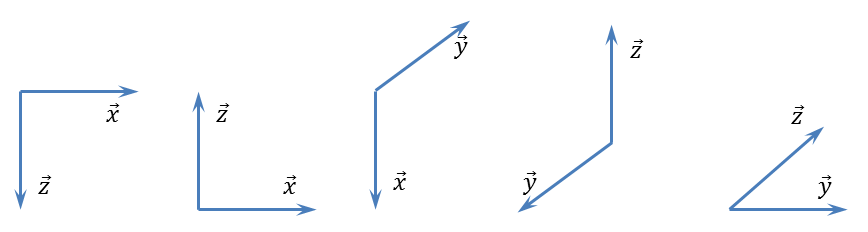
\includegraphics[width=.9\textwidth]{png/exo2}
\end{center}
\subparagraph{}
\textit{Exprimer les produits des vecteurs de base d'une base orthonormée directe.}
$$
\vect{x}\cdot\vect{y}
\quad
\vect{x}\wedge\vect{y}
\quad
\vect{y}\cdot\vect{z}
\quad
\vect{y}\wedge\vect{z}
\quad
\vect{x}\cdot\vect{z}
\quad
\vect{x}\wedge\vect{z}
$$

\ifthenelse{\boolean{prof}}{
\begin{corrige}
\end{corrige}
}{}

\subparagraph{}
\textit{Calculer le cosinus puis l'angle $\alpha$ formé par les vecteurs $\vect{V_1}=\left[\begin{array}{c}-1\\2\\2\end{array}\right]_{\mathcal{B}}$ et 
$\vect{V_2}=\left[\begin{array}{c}3\\-2\\3\end{array}\right]_{\mathcal{B}}$.}

\ifthenelse{\boolean{prof}}{
\begin{corrige}
\end{corrige}
}{}

\subparagraph{}
\textit{Calculer le sinus puis l'angle $\gamma$ formé par les vecteurs $\vect{V_1}=\left[\begin{array}{c}1\\4\\8\end{array}\right]_{\mathcal{B}}$ et 
$\vect{V_2}=\left[\begin{array}{c}-2\\5\\3\end{array}\right]_{\mathcal{B}}$.}

\ifthenelse{\boolean{prof}}{
\begin{corrige}
\end{corrige}
}{}

\subparagraph{}
\textit{Calculer l'angle entre $\vect{V}=10\vect{x}+8\vect{y}+6\vect{z}$ et le vecteur de base $\vect{x}$.}

\ifthenelse{\boolean{prof}}{
\begin{corrige}
\end{corrige}
}{}

\subsection*{Exercice 3}
\setcounter{subparagraph}{0}

\subparagraph{}
\textit{Représentez un repère orthonormé $\mathcal{R}=\left(O,\vect{x},\vect{y},\vect{z} \right)$ en vue orthogonale ($\vect{y}$ vertical, $\vect{x}$ horizontal, $\vect{z}$ vers <<nous>>), puis un repère orthonormé $\mathcal{R}_1=\left(O,\vect{x_1},\vect{y_1},\vect{z} \right)$ tel que $\alpha=\left(\vect{x},\vect{x_1}\right)$. Mettez un point $M$ tel que $\vect{OM}=a\vect{x_1}$ avec $a>0$.}

\ifthenelse{\boolean{prof}}{
\begin{corrige}
\end{corrige}
}{}

\subparagraph{}
\textit{Exprimer les composantes de $\vect{OM}$ en projection sur la base $\mathcal{B}$ liée au repère $\mathcal{R}$.}


\ifthenelse{\boolean{prof}}{
\begin{corrige}
\end{corrige}
}{}

\subparagraph{}
\textit{Exprimer $\vect{z}\wedge\vect{OM}$. Vous l'exprimerez en projection sur la base $\mathcal{B}$ puis dans $\mathcal{B}_1$ (utiliser plusieurs méthodes).}

\ifthenelse{\boolean{prof}}{
\begin{corrige}
\end{corrige}
}{}



\subsection*{Exercice 4}
\setcounter{subparagraph}{0}

On donne les coordonnées de trois points dans le repère orthonormé $\mathcal{R}  = \left(D,\vect{x},\vect{y},\vect{z} \right)$:
$$A : (3, 2, 0) \quad B : (0, 3, 2) \quad C : (2, 3, 0)$$
\subparagraph{}
\textit{Calculez les composantes du vecteur $\vect{V}$ de norme 1000 colinéaire à $\vect{AB}$ et de même sens.}

\ifthenelse{\boolean{prof}}{
\begin{corrige}
\end{corrige}
}{}

\subparagraph{}
\textit{Calculez le moment au point $A$ du pointeur $(D,\vect{D})$ où  $\vect{D}=(200,300,-100)_{\mathcal{B}}$.}

\ifthenelse{\boolean{prof}}{
\begin{corrige}
\end{corrige}
}{}

\subparagraph{}
\textit{Calculez le moment au point $E$ milieu de $AB$, du pointeur$(D,\vect{D})$.}

\ifthenelse{\boolean{prof}}{
\begin{corrige}
\end{corrige}
}{}

\subparagraph{}
\textit{Calculez le moment par rapport à l'axe $\delta$ (orienté de $A$ vers $B$) du pointeur $(D,\vect{D})$. }

\ifthenelse{\boolean{prof}}{
\begin{corrige}
\end{corrige}
}{}



\subsection*{Exercice 5}
\setcounter{subparagraph}{0}

\begin{minipage}[c]{.7\linewidth}
\subparagraph{}
\textit{On note $\mathcal{B}=(\vect{x},\vect{y},\vect{z})$, $\mathcal{B}_1=(\vect{x_1},\vect{y_1},\vect{z})$,  $\alpha=\left(\vect{x},\vect{x_1}\right)$, $\beta=\left(\vect{x_1},\vect{V} \right)$.}

\textit{Exprimer les composantes scalaires sous formes de colonnes du vecteur $\vect{V}$ en projection sur la base $\mathcal{B}_1$ puis sur la base $\mathcal{B}$ et ceci en fonction de la norme de $\vect{V}$ notée simplement $V$ et des angles orientés $\alpha$ et $\beta$. }
\end{minipage} \hfill
\begin{minipage}[c]{.29\linewidth}
\begin{center}
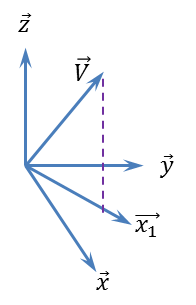
\includegraphics[height=4cm]{png/exo4_1}
\end{center}
\end{minipage}

\ifthenelse{\boolean{prof}}{
\begin{corrige}
\end{corrige}
}{}


\begin{minipage}[c]{.7\linewidth}
\subparagraph{}
\textit{Même question avec $\mathcal{B}=(\vect{x},\vect{y},\vect{z})$, $\mathcal{B}_1=(\vect{x_1},\vect{y_1},\vect{z})$,  $\alpha=\left(\vect{x},\vect{x_1}\right)$, $\beta=\left(\vect{y_1},\vect{V} \right)$.}
\end{minipage} \hfill
\begin{minipage}[c]{.29\linewidth}
\begin{center}
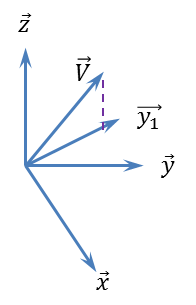
\includegraphics[height=4cm]{png/exo4_2}
\end{center}
\end{minipage}

\ifthenelse{\boolean{prof}}{
\begin{corrige}
\end{corrige}
}{}

\begin{minipage}[c]{.7\linewidth}
\subparagraph{}
\textit{Même question avec $\mathcal{B}=(\vect{x},\vect{y},\vect{z})$, $\mathcal{B}_1=(\vect{x_1},\vect{y_1},\vect{z})$,  $\alpha=\left(\vect{z},\vect{V}\right)$, $\beta=\left(\vect{x},\vect{x_1} \right)$.}
\end{minipage} \hfill
\begin{minipage}[c]{.29\linewidth}
\begin{center}
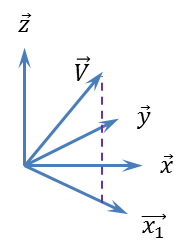
\includegraphics[height=4cm]{png/exo4_3}
\end{center}
\end{minipage}

\ifthenelse{\boolean{prof}}{
\begin{corrige}
\end{corrige}
}{}


\begin{minipage}[c]{.7\linewidth}
\subparagraph{}
\textit{Même question avec $\mathcal{B}=(\vect{x},\vect{y},\vect{z})$, $\mathcal{B}_1=(\vect{x_1},\vect{y},\vect{z_1})$,  $\alpha=\left(\vect{z_1},\vect{V}\right)$, $\beta=\left(\vect{z},\vect{z_1} \right)$.}
\end{minipage} \hfill
\begin{minipage}[c]{.29\linewidth}
\begin{center}
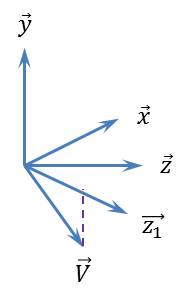
\includegraphics[height=4cm]{png/exo4_4}
\end{center}
\end{minipage}

\ifthenelse{\boolean{prof}}{
\begin{corrige}
\end{corrige}
}{}


\begin{minipage}[c]{.7\linewidth}
\subparagraph{}
\textit{Même question avec $\mathcal{B}=(\vect{x},\vect{y},\vect{z})$, $\mathcal{B}_1=(\vect{x},\vect{y_1},\vect{z_1})$,  $\alpha=\left(\vect{x},\vect{V}\right)$, $\beta=\left(\vect{z},\vect{z_1} \right)$.}
\end{minipage} \hfill
\begin{minipage}[c]{.29\linewidth}
\begin{center}
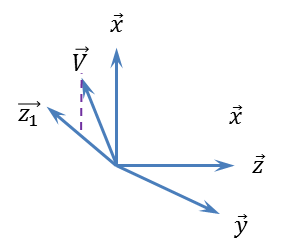
\includegraphics[height=4cm]{png/exo4_5}
\end{center}
\end{minipage}

\ifthenelse{\boolean{prof}}{
\begin{corrige}
\end{corrige}
}{}


\begin{minipage}[c]{.7\linewidth}
\subparagraph{}
\textit{Même question avec $\mathcal{B}=(\vect{x},\vect{y},\vect{z})$, $\mathcal{B}_1=(\vect{x_1},\vect{y_1},\vect{z})$,  $\alpha=\left(\vect{y_1},\vect{V}\right)$, $\beta=\left(\vect{y},\vect{y_1} \right)$.}
\end{minipage} \hfill
\begin{minipage}[c]{.29\linewidth}
\begin{center}
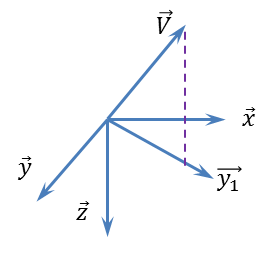
\includegraphics[height=4cm]{png/exo4_6}
\end{center}
\end{minipage}

\ifthenelse{\boolean{prof}}{
\begin{corrige}
\end{corrige}
}{}


\end{document}